% udokumenteret pumpeløsning 

\subsection{Udokumenteret pumpeløsning}
\label{sec:Udokumenteretpumpeloesning}

Alpha2 pumpen vidste sig i modultesten, se Projektdokumentationen afsnit 8.6 Alpha2 pumpe, ikke at være brugbar som vandpumpe til sprinkleren. Herunder beskrives den valgte prototype løsning.

Alpha2 pumpen byttes ud med en boremaskinepumpe til vand, denne pumpe drives af en 230 VAC boremaskine. Haveslangen forbindes med 1/2" slangetilslutning. 

Figur \ref{fig:boremaskinepumpe} viser boremaskinepumpen med tilhørende slangetilkoblinger. Boremaskinens kontakt tvinges ind vha. en strips og herved pumpes der med maksimal kraft så snart relæets kontaktsæt sluttes. 

%BOREMASKINEPUMPE BILLEDE
\begin{figure}[h]
  \centering
    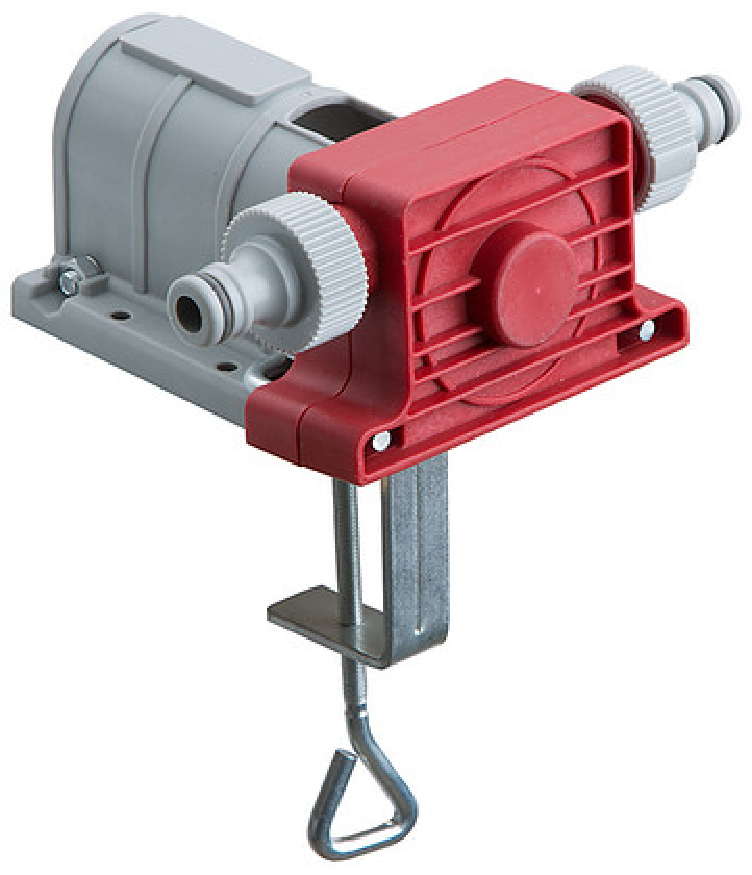
\includegraphics[width=0.3\textwidth]{Billeder/boremaskinepumpe}
    \caption{Boremaskinepumpe}
    \label{fig:boremaskinepumpe}
\end{figure}

Boremaskinepumpen er testet med vand og sprinkler og virker som forventet. 